\begin{quote}
    “ Les musées, gardiens et interprètes des témoignages initiaux de nos civilisations, seront les dépositaires des informations primaires qui devront être saisies et représentées sous de nouvelles formes. Leur rôle sera d'expliquer, d'explorer et d'élargir l'univers dans un nouveau langage multimédia. [...] Pour mener à bien cette mission, les gardiens de notre patrimoine vont devoir entreprendre dès maintenant les tâches suivantes : a) superviser le traitement numérique des informations  concernant ce patrimoine selon des normes garantissant la valeur de leur investissement ; 6) définir une politique de délivrance de licences protégeant l'utilisation des informations créées ; enfin c) explorer les possibilités de coopération  et de mise en commun  de l'information, sachant que les mondes culturel et social auxquels les collections sont associées peuvent être représentés selon les catégories courantes de la connaissance. La première tâche exige des responsables des musées  qu'ils entreprennent la saisie et l'informatisation des données qui se rapportent à leurs collections et à l'environnement auquel elles se réfèrent ; qu'en même temps ils constituent un fonds d'archives sonores et vidéo sur leurs collections en formats numériques  normalisés. Le Comité pour les échanges d'informations informatisées entre les musées (CIMI) a estimé que le meilleur moyen de préserver durablement ces données est de les indexer en utilisant le langage standard généralisé de balisage (SGML) (IS0 8879) et les mêmes modèles logiques de classement des données. Les systèmes informatiques contribuant à cette nouvelle documentation des collections doivent  être pleinement accordés à l'ensemble des activités du musée, de l'acquisition à l'exposition, et tenir compte des politiques et des procédures propres à chaque institution plutôt  que d'être greffés sur la  programmation existante et considérée comme une activité supplémentaire. 
[...]
Demain, des musées automatisés de ces données seront contraints de négocier avec  des centaines de musées. A l'heure actuelle, la  législation relative au traitement des droits sur les données numériques et au patrimoine culturel varie considérablement d'un pays à l'autre : c'est pourquoi, dans chaque pays, les musées doivent élaborer en commun des mécanismes de gestion de leurs droits dans ce domaine. Ils doivent également s'associer pour assurer la diffusion de ces matériels à l'extérieur de l'institution, sous peine de les voir tomber très vite dans le domaine public en vertu de la loi ou de l'usage [...] Surtout, l'institution  aurait perdu une occasion unique  d'ouvrir une brèche par laquelle les collections vont pouvoir envahir les maisons, les écoles, la rue, les lieux de travail. Dans cet espace, les interprétations et représentations des collections des musées vont devenir un instrument irremplaçable de sensibilisation du public à la culture et à la nature. Il reviendra aux musées du XXI siècle d'explorer ces possibilités, de proposer des expériences associant représentations abstraites et objets concrets dans une vision neuve, complexe, culturellement structurée et authentique du monde.”\footcite{Bearman_1994}
\end{quote} 
La question de la gestion des données culturelles s’est posée dès lors que les institutions se sont dotées de systèmes informatiques. Pour David Bearman, rédacteur en chef de la revue trimestrielle \textit{Archives and Museum Informatics}, les choses sont claires. Dans son article publié dans \textit{Museum International} en 1994, celui-ci décrit déjà les différentes étapes qu’il faudrait suivre pour garantir la qualité des données produites par les institutions culturelles et pour pouvoir les exploiter au mieux. Lors de la lecture de cet article, nous nous sommes immédiatement rendu compte que les règles évoquées faisaient encore partie de la réflexion aujourd'hui 30 ans plus tard. Parmi les règles qu’il évoque, la première règle est celle de la normalisation, la troisième est celle de la réflexion sur la mise en commun de ces données. \newline

Lors de notre stage au sein Service du numérique du ministère de la culture (SNUM), ces deux règles et donc éléments de réflexions ont été au centre de notre travail. 
L’objectif de notre stage à été de s’assurer que le modèle LIDO (Lightweight Information Describing Objects ) était un modèle de données conforme aux besoins très hétérogènes des partenaires culturels du ministère de la culture. Le modèle en question, que nous définirons plus en détail plus tard dans ce mémoire, est un schéma de données XML dérivé du CIDOC CRM (CIDOC Conceptual Reference Model), utilisé pour décrire et échanger  des collections muséales. Le modèle LIDO est celui qui va être utilisé pour servir de modèle d'échange de données entre les institutions et le ministère de la Culture. Les thèmes de la normalisation et de la mise en commun de l’information nous ont donc accompagné au long de notre projet. \newline

La mission du stage s’inscrit dans le cadre de la stratégie nationale d’agrégation des contenus culturels portée par le ministère de la Culture et sa mise en oeuvre:
L’agrégation des contenus culturels est un processus qui permet la collecte des liens vers les images et des métadonnées descriptives des œuvres détenues par des institutions culturelles. L’objectif est leur diffusion sur des portails, thématiques, régionaux, nationaux (comme par exemple la plateforme ouverte du patrimoine POP pour les données réglementaires autour des collections des Musées de France ou les données du patrimoine ou de l’inventaire) ou encore européens. C’est le cas d’Europeana \footcite{europeana}, un portail qui se propose de donner accès à plusieurs millions de contenus numérisés provenant d’institutions culturelles de toute l’Europe. Mais aussi, dans le futur, l’espace données culturel européen. Les espaces de données européens sont le produit de la stratégie data de la Commission européenne, pour rendre plus de données disponibles à la consultation et surtout à la réutilisation. Quatorze espaces de données européens sont en cours de spécification et de déploiement, chacun portant sur un domaine d'intérêt public, comme la santé, l’énergie ou les finances\footcite{eecd}.\newline

Le but du ministère, en collectant ces données culturelles, est d'offrir un point d’accès unique à une masse de contenus découvrables, pour faciliter une visibilité à toutes les échelles du patrimoine conservé par les institutions culturelles. 
L’agrégation devrait également permettre de rendre les données culturelles disponibles pour différentes réutilisations par d’autres acteurs que le milieu culturel, par exemple pour l’enseignement, la recherche ou encore le tourisme.
Le ministère de la Culture a pour mission d’agréger les données culturelles (notamment muséales et patrimoniales) de l’ensemble du territoire français, ne relevant pas du champ des données bibliographiques (livre, périodiques et imprimés qui sont pris en charge par l’agrégateur Gallica géré par la Bibliothèque Nationale de France) et des archives (prises en charge par l’agrégateur FranceArchives géré par le Service Interministériel des Archives de France).\newline 

Dans le cadre de cette mission, le ministère fait face à une grande diversité de formats et de protocoles utilisés par les différents établissements culturels. 
Cette diversité de pratiques a conduit à une fragmentation des données, chaque établissement développant ses propres méthodes de gestion de données en fonction de ses besoins spécifiques. Le terme de fragmentation des données définit un phénomène lors duquel les données sont dispersées et sont parfois trop différentes pour pouvoir les faire communiquer entre elles. 
C’est d’autant plus vrai que les établissements culturels font, pour la plupart, appel à des éditeurs de logiciels pour développer des solutions de gestion de collections ainsi que d'édition de leurs données. Ces éditeurs proposant chacun des solutions différentes et développant des outils de marché, cela participe à la fragmentation des données. Le paradoxe étant que beaucoup d'institutions sont très satisfaites de ce système car il leur permet d’accéder à des solutions personnalisées, répondant donc à leurs besoins principaux : ceux de la gestion en interne.\newline

Pendant de nombreuses années le ministère était organisé en silos avec une base/application par type de données, ce qui limitait la possibilité d'une approche transversale de la gestion des collections. Chaque proposition (applications ou autres) faite par le service, était développée pour répondre aux besoins spécifiques de chaque établissement, sans véritable souci de compatibilité ou d'interopérabilité \footnote{\emph{Interopérabilité }: Informatique
Capacité de matériels, de logiciels ou de protocoles différents à fonctionner ensemble et à partager des informations : Interopérabilité des réseaux téléphoniques. Source : Dictionnaire Larousse en ligne”}avec d'autres systèmes. La réorganisation et la création du Service du Numérique (SNUM) a remis à plat cette organisation et vise donc à casser ces silos et permettre l’interopérabilité des données tout en préservant les spécificités des différents métiers. L'objectif est de proposer une approche plus unie et une direction commune, permettant non seulement de rationaliser la collecte des données, mais aussi de standardiser les formats pour faciliter leur utilisation à des fins de recherche, de circulation, d'exposition ou d'exploitation par d'autres acteurs culturels.\newline 

C’est dans ce contexte de pratiques diverses que le besoin de normalisation des données s’est posé. En effet pour pouvoir mener à bien cette mission d'agrégation il faut réfléchir à un modèle de données qui soit commun aux données collectées pour permettre leurs circulation et ainsi exploitation. 
La normalisation est un processus essentiel pour transformer des informations hétérogènes en données homogènes, interopérables et exploitables. Cela s'inscrit dans une longue tradition de gestion de l'information dans les institutions culturelles, ainsi que dans tous les domaines qui ont besoin d’exploiter des données, quelles qu’elles soient. 
Depuis les premiers catalogues et livres d'inventaires jusqu'aux systèmes de classification modernes, la question de l'uniformisation des données a été un enjeu crucial. Normaliser, c'est avant tout rendre les données comparables, facilitant ainsi la recherche et l'interopérabilité entre les différents systèmes. \newline


Ce mémoire se propose donc d'explorer l'histoire et les enjeux de la normalisation des données culturelles, en s'intéressant particulièrement à son application dans le contexte des musées. Si les bibliothèques et les archives ont été pionnières en matière de normalisation, les musées ont longtemps accusé un certain retard. Aujourd'hui, cependant, ces institutions commencent à atteindre une certaine maturité dans ce domaine, notamment grâce à l'émergence d’initiatives de grande envergure, comme celle de l'agrégation des données muséales à l'échelle nationale. Parmi ces initiative sil nous faut mentionner l’harmonisation des données de la base Joconde, qui est le catalogue collectif des collections des musées de France. \newline Nous explorerons par la suite les standards et sytèmes de gestion de données utilisés aujourd'hui dans les muséee.\newline Pour finir, nous expliquerons comment nous avons vérifié que le modèle LIDO corresponde bien aux besoins de de normalisation essentiels pour mener à bien notre objectif d’agrégation des données culturelles françaises.

\begin{figure}[h!]
	\centerline{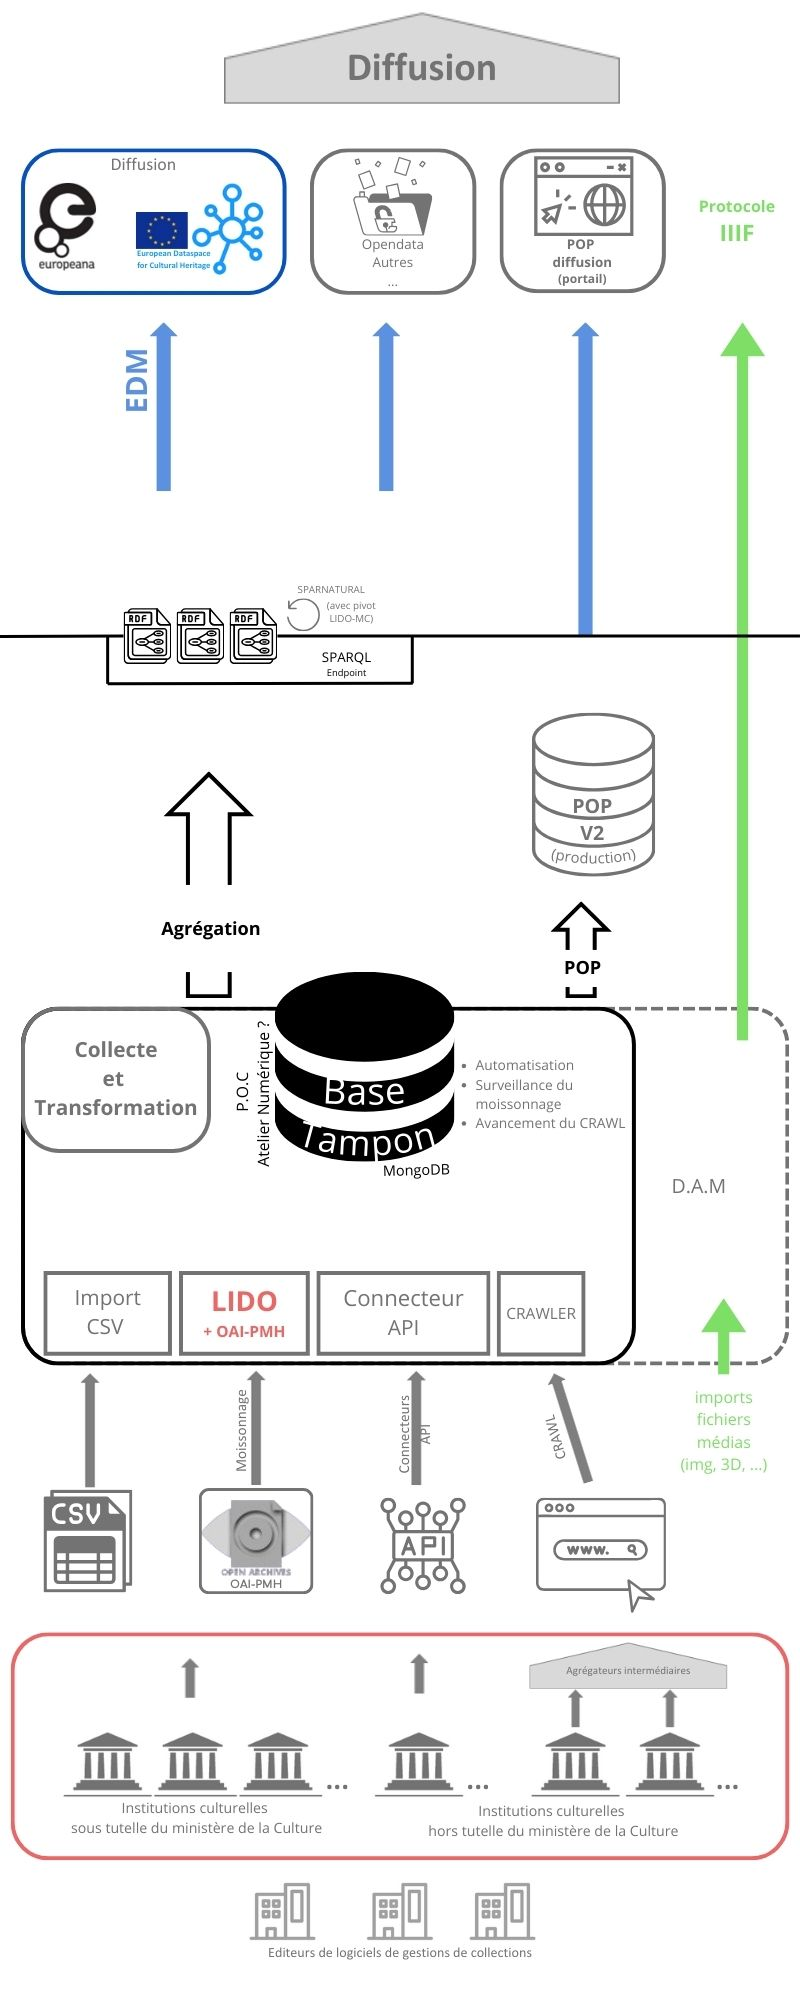
\includegraphics [height=0.8\textheight]{medias/schema_agregation.jpg} }
	\caption{Schéma illustrant la stratégie d'agrégation du Ministère de la Culture}
\end{figure}